\documentclass[ngerman,compress,hyperref={bookmarks}]{beamer}
\usepackage{beamerarticle}

\usetheme{Antibes}
\useoutertheme{infolines}

\usepackage[T1]{fontenc}
\usepackage[utf8x]{inputenc}

\usepackage{multirow}

\usepackage{colortbl}
\definecolor{darkgray}{rgb}{0.4, 0.4, 0.4}

\usepackage{wasysym}

\logo{
\includegraphics[height=1cm]{images/logoHAW}}
\usepackage{graphicx}

\usepackage{cite}

\usepackage{cancel}

\title[Aktive Messungen zur Validierung]{Aktive Messverfahren zur Topologievalidierung\\im Routing-Atlas}
\subtitle{Vortrag: Ringvorlesung Seminar}
\subject{Routing-Atlas, Topology}
\author{Andreas Krohn}
\institute[HAW]{Hochschule für Angewandte Wissenschaften Hamburg}
\date[WS 2012/13]{14. November 2012}

\begin{document}
\frame[plain]{\titlepage}

\section*{Agenda}
\begin{frame}{Agenda} \setcounter{tocdepth}{1} \tableofcontents[part=1] \setcounter{tocdepth}{3} \end{frame}

\part{Hauptteil}
\section{Intro}
\subsection{Motivation}
\begin{frame}[allowframebreaks]{Motivation}
  \begin{itemize}
    \item Internet ist kritische Infrastruktur
    \item Bestrebungen zur Kontrolle (Gesetzgeber, Contentindustrie,\ldots)
    \item Topologie nicht komplett bekannt
    \item Beteiligte nicht komplett bekannt
  \end{itemize}
  \framebreak
  Entwicklung eines Werkzeugs
  \begin{itemize}
    \item Zuordnung von Akteuren zu Ländern
    \item Modellierung der Topologie
    \item Visualisierung
    \item \color{darkgray}{Weitere Analysen\ldots}
  \end{itemize}
\end{frame}

\subsection{Routing-Atlas}
\begin{frame}[allowframebreaks]{Routing-Atlas}
  Ein Projekt der inet AG in Kooperation mit dem BSI \nocite{wsbh-envgi-12}
  \begin{itemize}
    \item Zusammenführung, Validierung und Analyse mehrerer Datenquellen
    \item Identifikation der Autonomen Systeme eines Landes
    \item Klassifikation der Autonomen Systeme nach Branche und Hierarchie
    \item Bildung des verbindenden Routinggraphen
    \item Visualisierung von Subgraphen
  \end{itemize}
  \vspace{0.1cm}
  {\small
  \begin{thebibliography}{}
    \bibitem{wsbh-envgi-12} ``Exposing a Nation-Centric View on the German Internet – A Change in Perspective on the AS Level''
    \newblock Matthias Wählisch, Thomas C. Schmidt, Markus de Brün, Thomas Häberlen\\
    \newblock In Proc. of the 13th Passive and Active Measurement Conference (PAM), volume 7192 of LNCS, page 200–210, Berlin Heidelberg, 2012. Springer-Verlag.\\[-20pt]
  \end{thebibliography}}
  \framebreak
  \begin{columns}[c]
    \begin{column}{0.5\textwidth}
      \begin{figure}
        \label{asgraphs}
        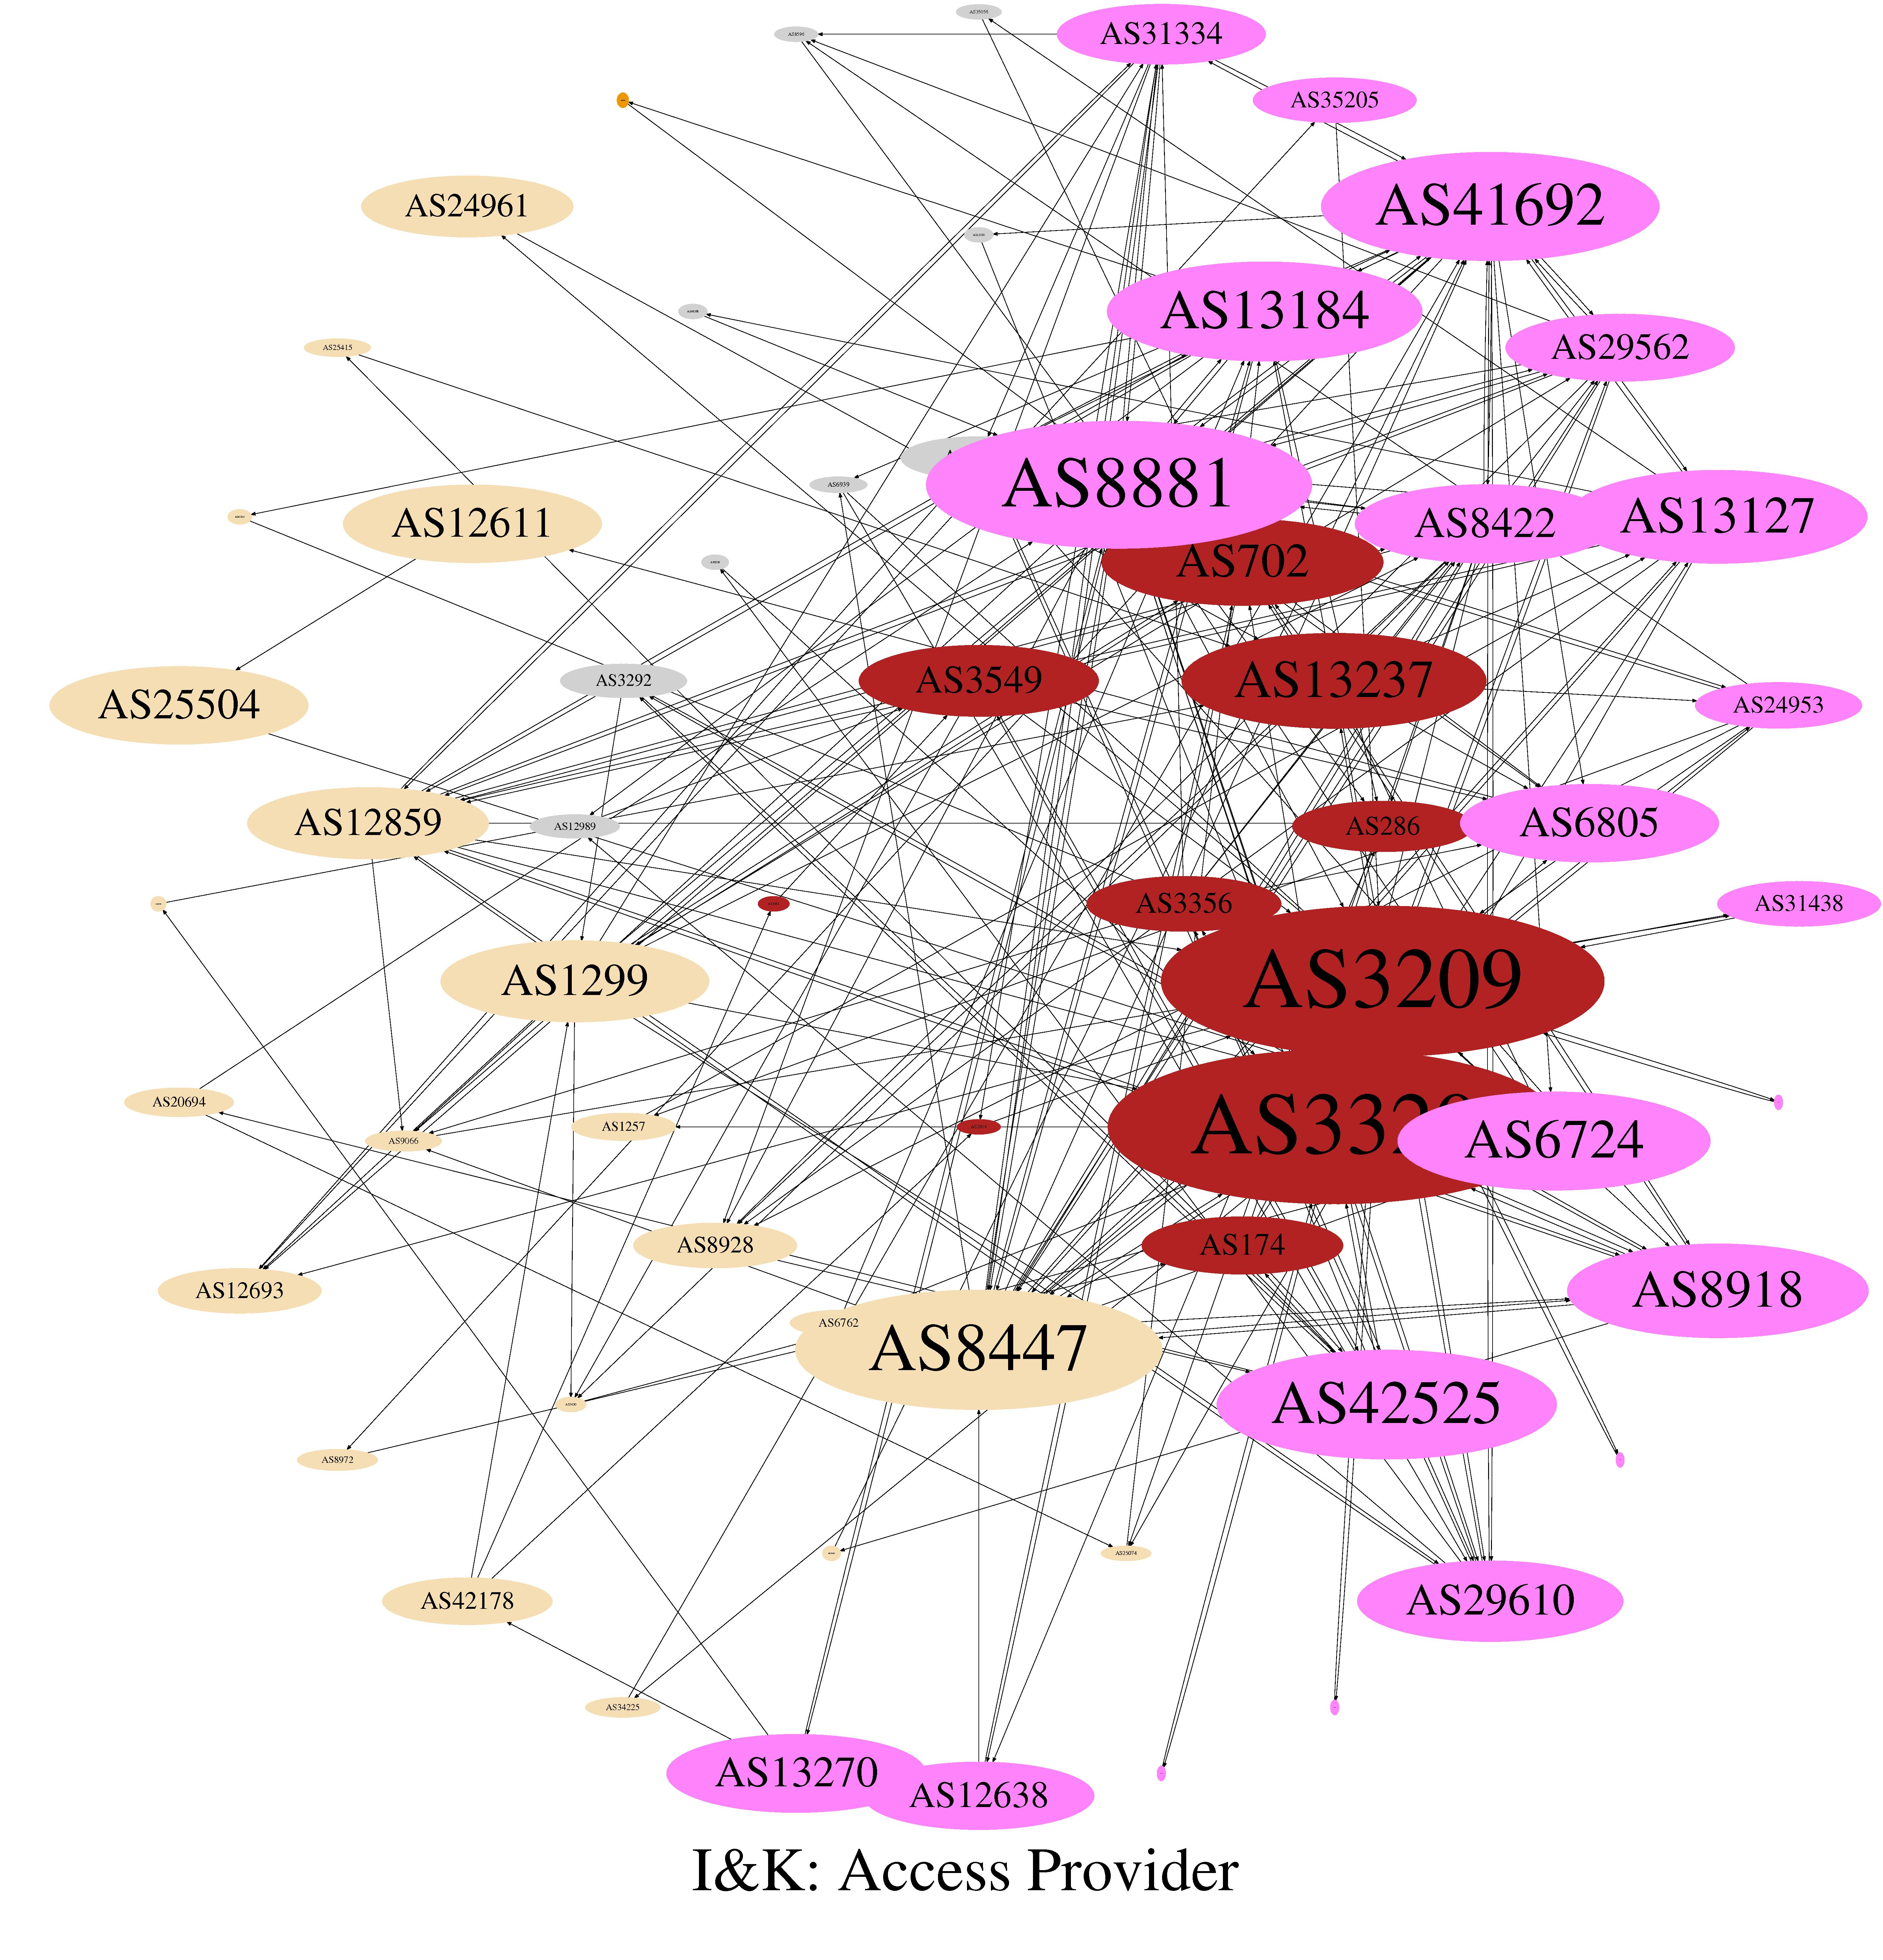
\includegraphics[width=1\textwidth]{images/asgraph_cat5-pos-betweenness}
      \end{figure}
    \end{column}
    \begin{column}{0.5\textwidth}
      \begin{figure}
        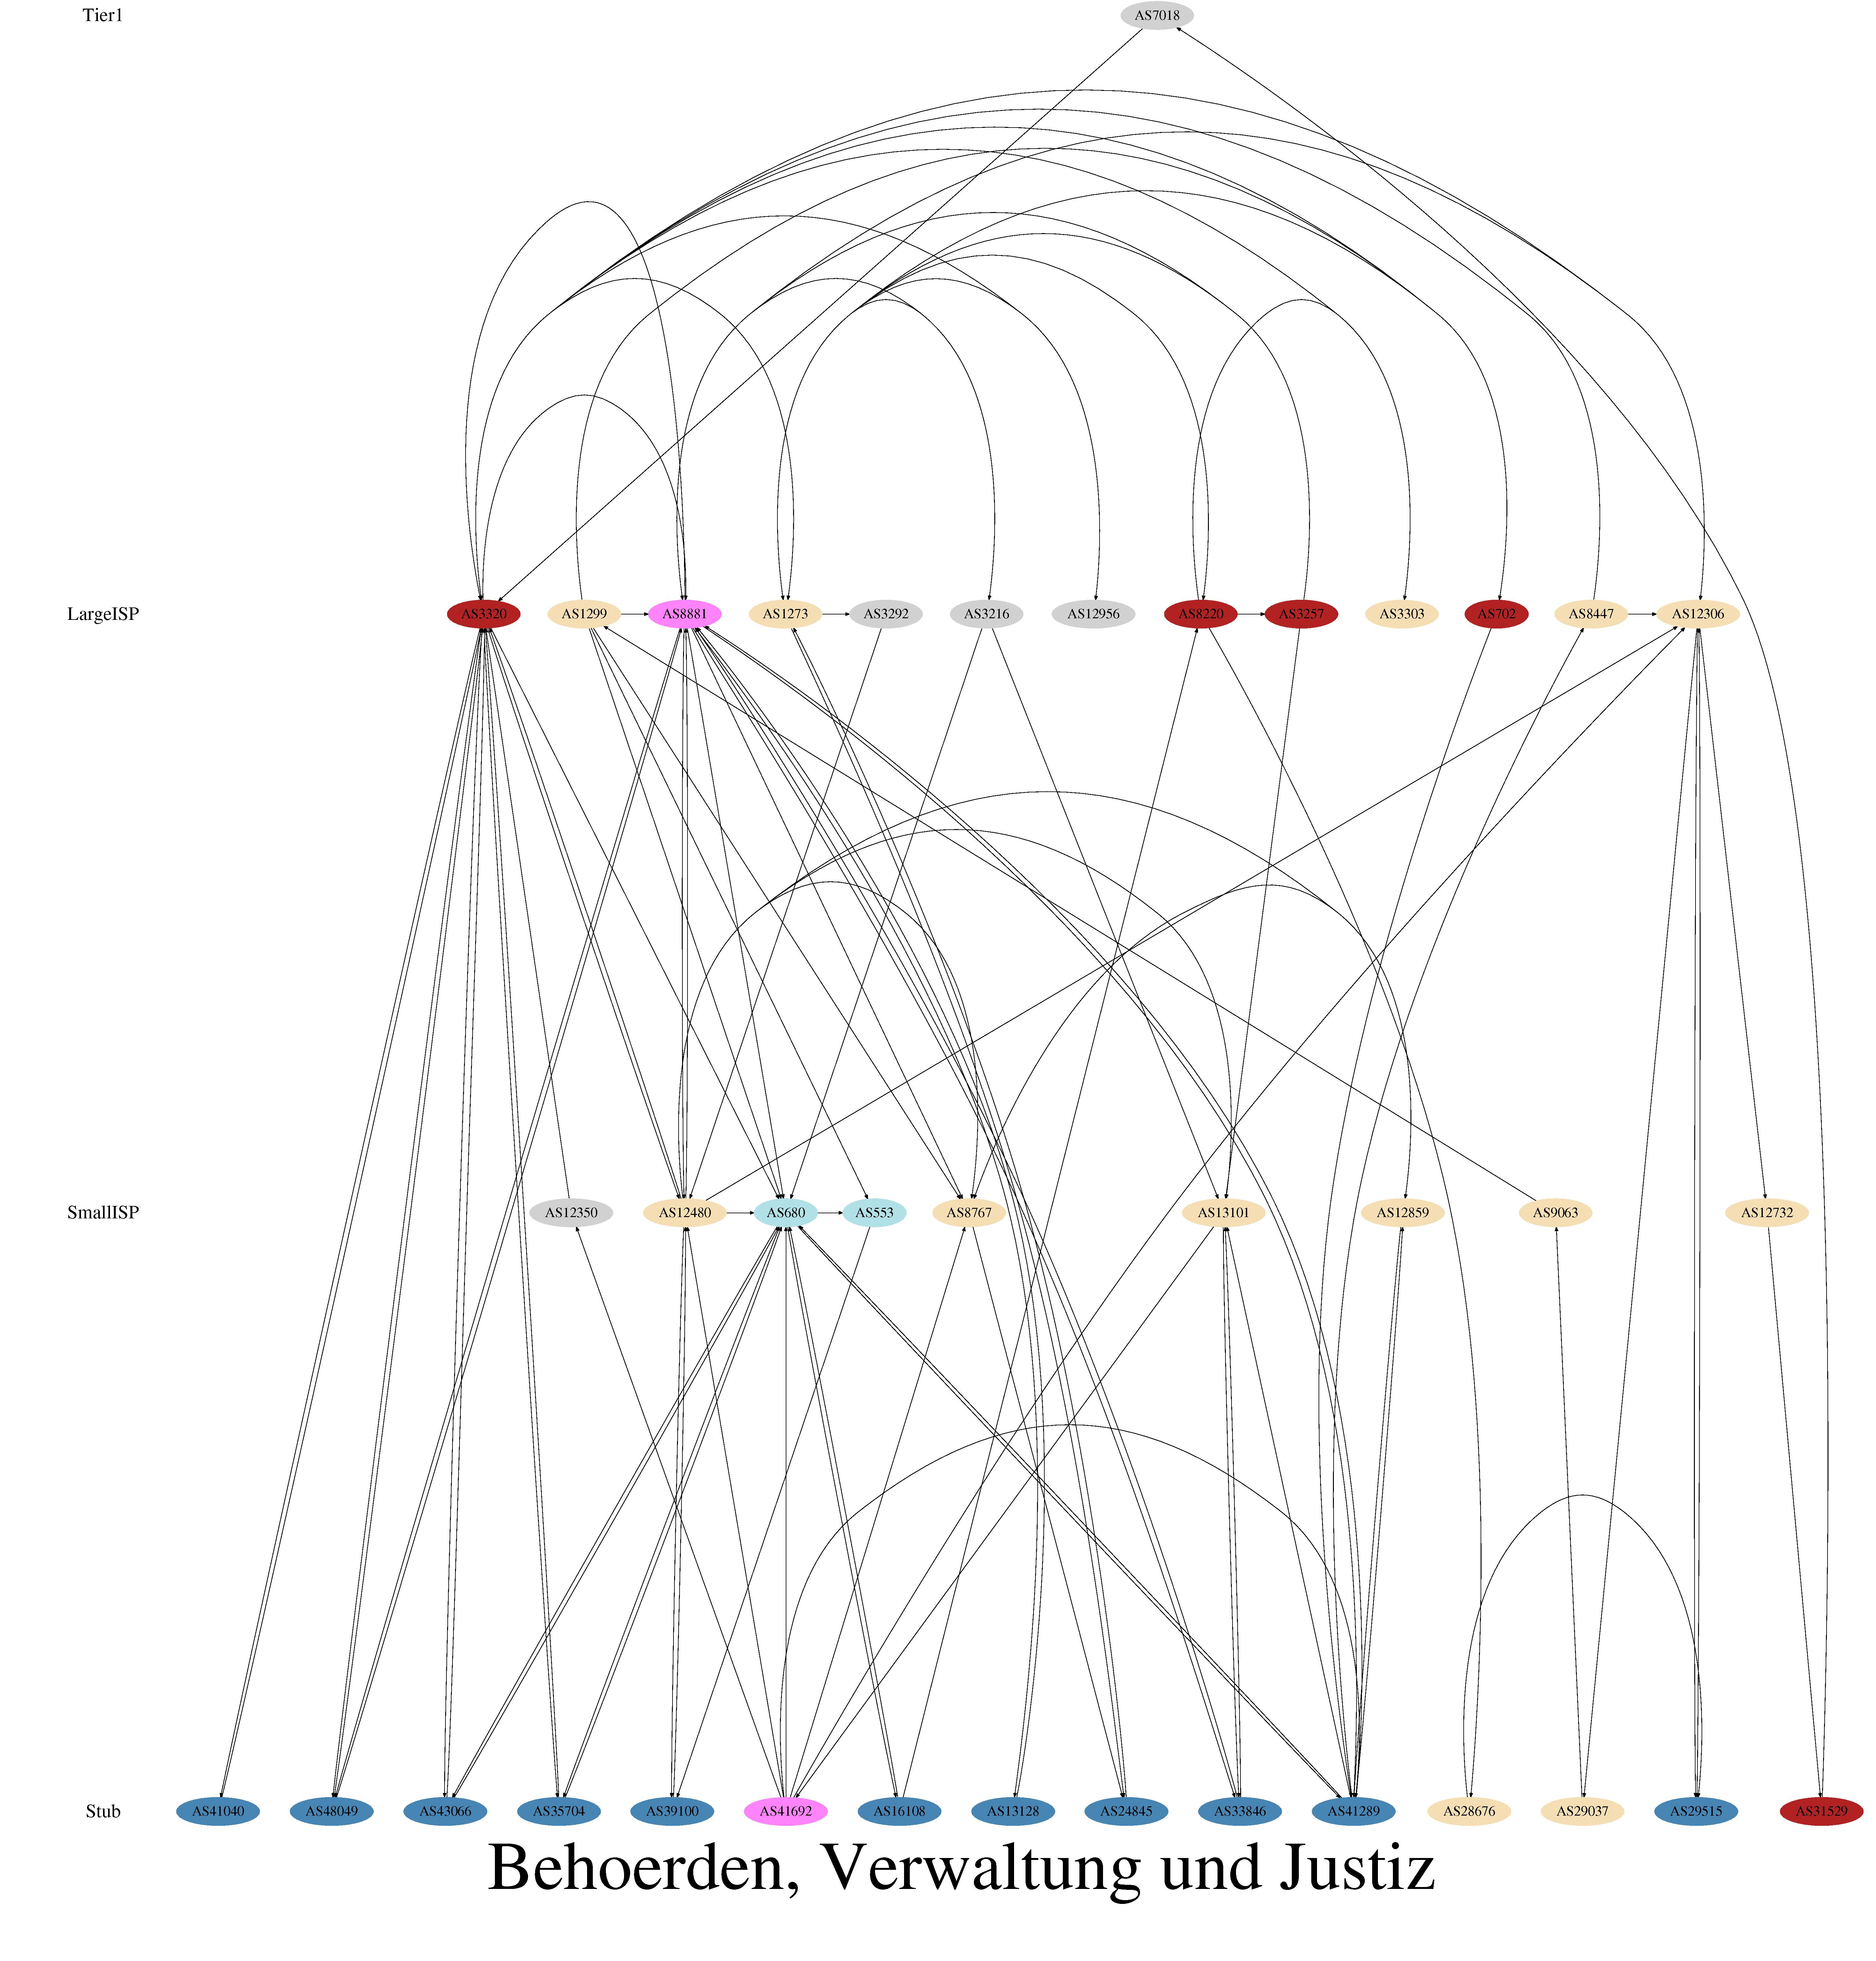
\includegraphics[width=1\textwidth]{images/asgraph_cat9-dot}
      \end{figure}
    \end{column}
  \end{columns}
\end{frame}

\section{Rückblick}
\subsection{AW 1}
\begin{frame}{Anwendungen 1 \cite{KrohnAW1}}{Vorstellung des Projekts Routing-Atlas}
  Aktueller Stand\\
  \begin{itemize}
    \item Identifikation des „deutschen Internets“
    \item Bildung des verbindenden AS Graphen über shortest path matrix
    \item Visualisierung
  \end{itemize}
  \vspace{0.3cm}
  Problemstellung\\
  \begin{itemize}
    \item Als Datenquelle verwendetes Projekt eingestellt
    \item Teils noch manuelle Schritte erforderlich
  \end{itemize}
  \vspace{0.3cm}
  Ziel\\
  \begin{itemize}
    \item Ersatz für shortest path matrix \cite{Winter:2009:MIR:1577959.1577976}
    \item Regelmäßige Bereitstellung aktueller Analysen
  \end{itemize}
\end{frame}

\subsection{AW2}
\begin{frame}{Anwendungen 2 \cite{KrohnAW2}}{Vorstellung vergleichbarer Arbeiten}
  Datensammlung, Topologieinferenz und -analyse
  \begin{itemize}
    \item Sammlung von BGP Tabellen und -Updates und Nutzung der IRR-Datenbanken \cite{Zhang:2005:CIA:1052812.1052825}
    \item Inferenz von AS Linktypen und Einteilung in tier1, non-tier1-transit und stub \cite{Gao:2001:IAS:504611.504616}
    \item Berechnung einer möglichst umfassenden Topologie \cite{Winter:2009:MIR:1577959.1577976}
    \item Entdeckung weiterer Peerings mittels traceroute \cite{Augustin:2009:IM:1644893.1644934}
  \end{itemize}
\end{frame}

\section{Work in Progress}
\subsection{Projekt1}
\begin{frame}[allowframebreaks]{Projekt1}
  Ursprüngliches Ziel: Aktualisierung der Topologiemodellierung
  \begin{itemize}
    \item Versuchsweise Implementierung von single- und all-pair-shortest-path Algorithmen
    \item Untersuchung zu Laufzeitverhalten und Speicherverbrauch
    \item Fazit: Es gibt Tools, die das besser können\\
    \hspace{0.3cm}z.B. \url{http://www.r-project.org/}
  \end{itemize}
  Nebenbei:
  \begin{itemize}
    \item Validierung der Länderzuordnung mittels GeoIP Datenbank
  \end{itemize}
  \framebreak

  Jetzt: Validierung und Ergänzung der Topologiemodellierung
  \begin{itemize}
    \item Passive Daten abhängig vom Standort \& oft wenig Informationen über Rückweg
    \item Über Kontakte Topologieausschnitt verifizieren (nachfragen)
    \item Mittels aktiver Verfahren diesen Ausschnitt nachvollziehen
    \item Vergleich mit modellierter Topologie
    \item Topologie um Ergebnisse aktiver Messungen ergänzen, sofern sich diese als brauchbar erweisen
  \end{itemize}
  \begin{figure}
    \label{graph_diff}
    \includegraphics[width=.6\textwidth]{images/graph_diff}
  \end{figure}
\end{frame}

\subsection{Aktives Messen}
\begin{frame}{Aktives Messen}
  Vorhanden
  \begin{itemize}
    \item Peering am BCIX
    \item Wissen über Peerings einiger Mitglieder
    \item Modellierte Topologie aus BGP Tabellen und Updates
  \end{itemize}
  Ziel
  \begin{itemize}
    \item Nachweis möglichst vieler Peerings mittels aktivem Messen
%     \begin{itemize}
%       \item Mit direktem Zugang zum IXP
%       \item Später: Looking Glas Server im Umfeld des IXP
%     \end{itemize}
    \item Vergleich der Peerings in modellierter Topologie, Messergebnis und Realität
    \item Integration der Messergebnisse in den Routing-Atlas
  \end{itemize}
\end{frame}

\begin{frame}{traceroute „durch“ IXPs}
  Angelehnt an „IXPs: Mapped?“ \cite{Augustin:2009:IM:1644893.1644934}
  \begin{itemize}
    \item Mitglieder und Präfixe am BCIX ermitteln
    \item traceroute in die Umgebung
    \item Peerings nachweisen
  \end{itemize}
  \begin{figure}
    \label{augustin_ixp}
    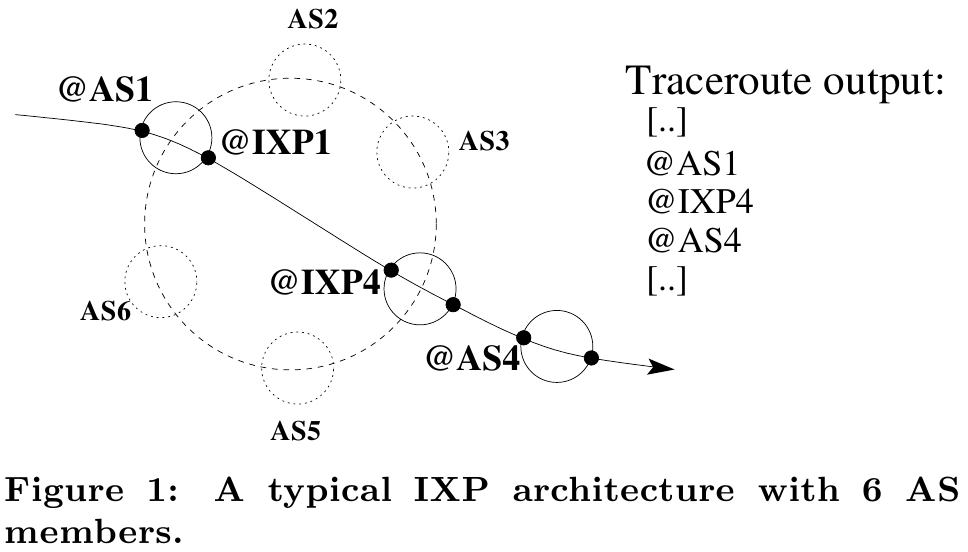
\includegraphics[width=1\textwidth]{images/augustin_ixp}
  \end{figure}
\end{frame}

\begin{frame}{reverse-traceroute}
  Angelehnt an „Reverse traceroute“ \cite{Katz-Bassett:2010:RT:1855711.1855726}
\end{frame}

\section{Ausblick}
\begin{frame}{Ausblick}
  Projekt 2
  \begin{itemize}
    \item in Projekt 1 entwickelte Messergebnisse in Routing-Atlas integrieren
  \end{itemize}
  \vspace{0.3cm}
  Außerdem
  \begin{itemize}
    \item zunächst Projekt 1 abschließen
    \item Thema der Masterarbeit konkretisieren
  \end{itemize}
\end{frame}

\part{Ende}
\section{kthxbye}
\begin{frame}[plain]{Ende}
\begin{columns}[t]
\begin{column}{0.5\textwidth}
 \begin{center}
 \vspace{1cm}
 Vielen Dank für die Aufmerksamkeit\\
 \vspace{1.5cm}
 Fragen\ldots?
 \end{center}
\end{column}
\begin{column}{0.5\textwidth}
 \vspace{-1cm}
 \begin{figure}
  \label{asngraphs2}
  \includegraphics[width=\textwidth]{images/asgraph_cat4-pos}
 \end{figure}
\end{column}
\end{columns}
\end{frame}

\section{Literatur}
\begin{frame}[plain, allowframebreaks]{Literatur}
\scriptsize
% \bibliographystyle{alpha}    % -> [AAAyy]
% \bibliographystyle{IEEEtran} % -> [n]
\bibliographystyle{apalike}
\bibliography{folien}
\end{frame}

\section{Bildquellen}
\begin{frame}[plain]{Bildquellen}
  \scriptsize
%   \tiny
  \begin{table}
    \begin{tabular}{ c p{0.8\textwidth} }
      Seite & Quelle \\ \hline
      \pageref{asgraphs}, \pageref{asngraphs2} & \url{http://inet.cpt.haw-hamburg.de/projects/routing-atlas/}\\ \hline
      \pageref{augustin_ixp} & \url{http://www-rp.lip6.fr/~augustin/ixp/imc2009.pdf} \\ \hline
    \end{tabular}
  \end{table}
\end{frame}

\end{document}
